\documentclass[12pt]{report}

% includes
\usepackage{geometry}           % page size
\usepackage[utf8]{inputenc}     % encoding
\usepackage{palatino}           % font
\usepackage[romanian]{babel}    % language
\usepackage{graphicx}           % images
\usepackage{indentfirst}        % indentation
\usepackage[nottoc]{tocbibind}  % table of contents style
\usepackage[unicode]{hyperref}  % references from the table of contents
\usepackage{dirtree} % for a simple directory tree
\usepackage{listings}

\lstset{
language=Java,
basicstyle=\small\sffamily,
breaklines=true,
breakatwhitespace=false,
numbers=left,
numberstyle=\tiny,
frame=single,
columns=fullflexible,
showstringspaces=false
}

% includes options
\geometry{  a4paper,            % scientific thesis standard
            left=3cm,
            right=2cm,
            top=2cm,
            bottom=2cm,
 }
\graphicspath{{images/}}        % path where the images are located
\setlength{\parindent}{1cm}     % paragraph indentation

% other options
\linespread{1.5}                % space between lines
\renewcommand*\contentsname{Cuprins}    % table of contents name

% the document content
\begin{document}
    % macros (global)
    \newcommand{\university}    {Universitatea "Alexandru-Ioan Cuza" din Iași}
\newcommand{\universityg}   {Universității "Alexandru-Ioan Cuza" din Iași} % genitive
\newcommand{\faculty}       {Facultatea de informatică}
\newcommand{\facultyg}      {Facultății de informatică} % genitive
\newcommand{\speciality}    {informatică}
\newcommand{\promotion}     {2019}                                  %<---------

\newcommand{\thesistype}    {Lucrare de licență}
\newcommand{\thesistitle}   {Generare Procedurală Folosind Modele Markov}    %<---------

\newcommand{\authorlast}    {Loghin}                               %<---------
\newcommand{\authorfirst}   {Alexandru}
\newcommand{\authornamefl}  {\authorfirst \space \authorlast} % first name first
\newcommand{\authornamelf}  {\authorlast \space \authorfirst} % last name first
\newcommand{\authorbirth}   {26 decembrie 2019}                      %<---------
\newcommand{\authoraddress} {România, jud. Iași, mun. Pașcani, Ale. 1 Decembrie 1918, nr. 1, bl. C17, sc.B et. 1, ap. 27} %<---------
\newcommand{\authorcnp}     {1971226225902}                         %<---------

\newcommand{\session}       {iulie, 2019}                       %<---------
\newcommand{\coordinator}   {Conf. Dr. Anca Vitcu}               %<---------

\newcommand{\dottedline}    {............................}
    
    % front-matter
    \pagenumbering{gobble}
    
    % define the cover page
\begin{titlepage}
    \begin{center}
        % the university and faculty
        \large
        \MakeUppercase{\university}
        
        \LARGE
        \textbf{\MakeUppercase{\faculty}}
        
        % the faculty logo
        \vspace{1cm}
        
\includegraphics[width=0.3\textwidth]{logoFii.png}
        
        % thesis title
        \vspace{1cm}
        \Large
        \MakeUppercase{\thesistype}
        
        \vspace{0.5cm}
        \LARGE
        \textbf{\thesistitle}
        
        % author
        \vspace{2cm}
        \Large
        propusă de
        
        \vspace{0.5cm}
        \LARGE
        \textbf{\authornamefl}
        
        % session
        \vfill
        \Large
        \textbf{Sesiunea:} \session
        
        % scientific coordinator
        \vspace{2cm}
        \Large
        Coordonator științific
        
        \vspace{0.5cm}
        \LARGE
        \textbf{\coordinator}
    \end{center}
\end{titlepage}
    % define the title page
\begin{titlepage}
    \begin{center}
        % the university and faculty
        \large
        \MakeUppercase{\university}
        
        \LARGE
        \textbf{\MakeUppercase{\faculty}}
        
        % thesis title
        \vspace{8cm}
        \huge
        \textbf{Generare Procedurală \linebreak  Folosind Modele Markov}
        
        % author
        \vspace{2cm}
        \LARGE
        \textbf{\authornamefl}
        
        % session
        \vfill
        \Large
        \textbf{Sesiunea:} \session
        
        % scientific coordinator
        \vspace{4cm}
        \Large
        Coordonator științific
        
        \vspace{0.5cm}
        \LARGE
        \textbf{\coordinator}
    \end{center}
\end{titlepage}
    \vspace*{\fill}

\begin{flushright}
    Avizat, \\
    Îndrumător lucrare de licență, \\
    \coordinator. \\
    Data: \dottedline \hspace{1cm} Semnătura: \dottedline
\end{flushright}

\vspace{1cm}
\begin{center}
    \large
    \textbf{Declarație privind originalitatea conținutului lucrării de licență}
\end{center}

Subsemnatul \textbf{\authornamelf} domiciliat în \textbf{\authoraddress}, născut la data de \textbf{\authorbirth}, identificat prin CNP \textbf{\authorcnp}, absolvent al \facultyg, \textbf{\faculty} specializarea \textbf{\speciality}, promoția \promotion, declar pe propria răspundere cunoscând consecințele falsului în declarații în sensul art. 326 din Noul Cod Penal și dispozițiile Legii Educației Naționale nr. 1/2011 art. 143 al. 4 și 5 referitoare la plagiat, că lucrarea de licență cu titlul \textbf{\thesistitle} elaborată sub îndrumarea domnului \textbf{\coordinator}, pe care urmează să o susțin în fața comisiei este originală, îmi aparține și îmi asum conținutul său în întregime.

De asemenea, declar că sunt de acord ca lucrarea mea de licență să fie verificată prin orice modalitate legală pentru confirmarea originalității, consimțind inclusiv la introducerea conținutului ei într-o bază de date în acest scop.

Am luat la cunoștință despre faptul că este interzisă comercializarea de lucrări științifice în vederea facilitării falsificării de către cumpărător a calității de autor al unei lucrări de licență, de diplomă sau de disertație și în acest sens, declar pe proprie răspundere că lucrarea de față nu a fost copiată ci reprezintă rodul cercetării pe care am întreprins-o.

\begin{flushright}
    Data: \dottedline \hspace{6cm} Semnătura: \dottedline
\end{flushright}

\vspace*{\fill}
\pagebreak
    \vspace*{\fill}
\begin{center}
    \large
    \textbf{Declarație de consimțământ}
\end{center}

Prin prezenta declar că sunt de acord ca lucrarea de licență cu titlul \textbf{\thesistitle}, codul sursă al programelor și celelalte conținuturi (grafice, multimedia, date de test, etc.) care însoțesc această lucrare să fie utilizate în cadrul \facultyg.

De asemenea, sunt de acord ca \faculty \space de la \university, să utilizeze, modifice, reproducă și să distribuie în scopuri necomerciale programele-calculator, format executabil și sursă, realizate de mine în cadrul prezentei lucrări de licență.

\begin{flushright}
    Absolvent \textbf{\authornamefl} \\
    \vspace{0.5cm}
    Data: \dottedline \hspace{6cm} Semnătura: \dottedline
\end{flushright}
\vspace*{\fill}
\pagebreak
    
    % table of contents
    \tableofcontents
    
    % chapters
    \setcounter{page}{1}
    \pagenumbering{arabic}
    
    \chapter*{Motivație} 
\addcontentsline{toc}{chapter}{Motivație}

Datorita pasiunii mele pentru \textit{gamedev} și algoritmică am decis să realizez o modalitatea de a genera procedural un mediu căt mai diversificat. Folosirea modelelor Markov a venit din necesitatea de a scăpa cumva de metoda clasică prin care se genereaza un șir de obiecte într-un mod aleator iar apoi se încearcă validarea acesteia după anumite constrângeri. Folosind acest model stocastic putem controla apariția unei anumite subsecvențe prin stabilirea unei anumite probabilități de a se produce așadar eliminând cu totul pasul de validare.\par

Scopul principal al proiectului a fost dezvoltarea unei librări ce ușurează procesul de generare. De asemenea a fost nevoie și de un sistem ce facilitează plasarea obiectelor în mediul 3D , modelul Markov fiind folosit doar ca și generator. Odată funcționale mi-am îndreptat atenția asupra interfeței grafice și a interacțiunii dintre jucător și joc.\par

Datorită motorului grafic folosit și a instrumentelor de care dispune , timpul necesar pentru crearea jocului a fost îmbunătățit substanțial. De asemena cu prilejul acestei aplicații am avut posibilitatea de a aprofunda și testa diferite tehnici de randare și postprocesare. Câteva dintre aceste elemente includ SSR \footnote{Screen Space Reflection} , lumina volumetrică  , reflexii în timp real , corectare de culoare și multe altele.\par

Odată cu finalizarea acestei aplicații , din cauza naturii sale \textit{open-source} , se va putea folosi librăria creată în cadrul acesteia pentru orice tip de proiect fără constrăngeri , fiind ușor adaptabilă pentru orice sarcină ce necesită generare procedurală , de la muzică până la construcția unui mediu virtual, librăria find ușor de folosit și axata pe eficiență.\par
    \chapter*{Introducere} 
\addcontentsline{toc}{chapter}{Introducere}

Având în vedere necesitatea creării unor medii căt mai versatile ce respectă anumite condiții sau restricții fizice s-au dezvoltat anumite tehnici pentru a facilita construcția automată și randomizată a oricărui element ce intră în componența unui joc , de la modele tridimensionale până la coloana sonoră.\par

Am decis așadar să încerc o abordare nouă , folosindu-mă de un model Markov ce a fost antrenat sa respecte anumite reguli pentru a genera spațiul 3D. Scopul acestei lucrări este de a aduce o nouă perspectivă asupra generării procedurale și de a demonstra validitatea acestei abordări.\par

Tema lucrării s-a ivit din cauza necesității de adaptare rapidă a condițiilor folosite pentru generarea obiectelor din componența unui joc.Unul din avantajele acestei abordări este flexibilitatea oferită de modelul Markov fiind capabil sa adapteze constrăngerile folosite la generare cu o simpla reantrenare a modelului.\par

Aplicația prezentă este construită folosind un motor grafic peste care am dezvoltat o librărie capabilă să reprezinte un model Markov și să îl antreneze. Folosindu-mă de această librărie , pot genera o secvență de obiecte ce încearcă să respecte fidel constrăngerile folosite la antrenare.\par

Procesul de generare procedurală este compus din două etape. Generarea obiectelor și plasarea lor convenabil în șpațiul virtual. Am încercat în special să decuplez cele două etape pentru o mai bună modularizare și o coeziune ridicată. Cele două sisteme lucrează independent unul față de celălalt , relația dintre cele două find una de agregare.

Cele două sisteme sunt puse în funcțiune pentru a genera în timp real mediul pentru jucător , mediu ce este împărțit în trei zone de interes , urbana , rurală și desertică. De asemenea pentru a adauga complexitate se alternează între trei tipuri de platforme ce simulează un drum drept , cu viraj la stănga sau cu viraj la dreapta.\par
    
    \chapter{Aspecte teoretice}

\section{Preambul}

În domeniul probabilităților un model Markov este folosit pentru a modela un sistem ce se schimbă într-un mod aleator. De obicei acesta ține cont doar de starea curentă și nu depinde de evenimentele aleatoare, acest lucru numindu-se și prorietatea Markov. Ulterior s-au dezvoltat modele ce au un așa numit ordin, extinzând astfel numărul de stări de care se ține cont în cadrul modelului.\par

De obicei există o separație clară între tipurile de modele Markov, criteriul folosit este disponibilitatea de a observa sau nu stările modelului. Așadar rezultă două mari categorii, sisteme cu stări complet observabile, din care fac parte lanțurile Markov și sisteme cu stări parțial observabile, cel mai cunoscut sistem fiind modelul Markov cu stări invizibile sau HMM \footnote{Hidden Markov Model}. Pe langă aceste modele prezentate, s-au dezvoltat și anumite derivate fiecare cu avantajele sale demonstrând astfel flexibilitatea și capacitatea de modelare a acestor sisteme.\par

În mare parte această teză se axează în jurul parții discrete a acestor modele, numărul de stări/observații find finit numărabile și ușor de caracterizat dar există și o ramură ce se ocupă cu partea continuă a acestor modele, fiecare abordare avănd avantajele și dezavantajele ei.\par

Legat de partea practică, de-a lungul timpului aceste modele au fost folosite în foarte multe domenii de la bioinformatică până la lingvistică computațională. O aplicație foarte importantă a acestor modele este recunoașterea vocală, modelele Markov fiind standardul folosit în industrie pentru asistenții personali ca \textit{Siri} și \textit{Alexa}.\par

\section{Modele Markov cu stări invizibile}

Acest model statistic este caracterizat în principal de faptul că stările interne sunt ascunse de un privitor exterior. Tot ce se poate observa în cadrul acestui model este emisia unor etichete sau obiecte 
$\{v_{1},v_{2},v_{3},\dots,v_{n}\}$ dintr-o mulțime notată pe scurt $V$. Acest lucru complică în general structura modelului și algortimii ce folosesc acest sistem. \par

Un avantaj direct este creșterea capacității de expresivitate, putând modela mai fidel datele, datorită eliminării necesității de a cunoaște toate stările evenimentului.\par

Pentru a caracteriza concret și complet acest model avem nevoie de un \textit{5-uplu} $ HMM = (\textbf{S},\textbf{V},\textbf{A},\textbf{B},\pi)$ ce desemnează astfel : \par
\begin{itemize}
\item{$\textbf{S} = \{S_{1},S_{2},\dots,S_{N}\}$ mulțimea ce desemnează numărul de stări ascunse din model, avand un numar de $N$ elemente. Starea relativa la timpul $t$ se va nota ca si $q_{t}$.}
\item{$\textbf{V} = \{V_{1},V_{2},\dots,V_{M}\}$ , cele $M$ etichete observabile.}
\item{$\textbf{A} = \{a_{ij}\}$ unde $a_{i,j} = P(q_{t+1} = S_{j} | q_{t} = S_{i}) , 1 \leq i , j \leq N$ , reprezentând distribuția de probabilitea asociată tranzițiilor între stări.}
\item{$\textbf{B} = \{b_{i}(k)\}$ unde $b_{i}(k) = P(V_{k}\ la\ timpul\ t\ | q_{t} = S_{i}), 1 \leq i \leq N , 1 \leq k \leq M$, ce caracterizează distribuția de probabilitate asociată emiterii unui element din $V$ în starea $i$.}
\item{$\pi = \{\pi_{i}\}$ unde $\pi_{i} = P(q_{1} = S_{i}) , 1 \leq i \leq N$, folosit inițial pentru a stabili prima stare din model și anume $q_{1}$.}
\end{itemize}
\par

În general modul de funcționare a acestui model poate fi descris foarte ușor cu o bucată de pseudocod:

\begin{lstlisting}[mathescape=true]
t $\gets$ 1;
stare $\gets$ alege o stare $S_{i}$ cu probabilitate $\pi_{i}$;
repeta la infinit
	stare $\gets$ alege o noua stare $S_{j}$ de tranzitie de la starea $S_{i}$ cu probabilitate $a_{ij} \in \textbf{A}$;
	afiseaza observatia $V_{k}$ cu probabilitatea $b_{i}(k)\in \textbf{B}$;
	t $\gets$ t + 1;
\end{lstlisting}

Uneori printre alte publicații de specialitate modelul poate fi descris prin specificarea parametrilor $N,M$ și cele trei distribuții de probabilitate notate astfel $\lambda = \{\textbf{A},\textbf{B},\pi\}$.\par
\vspace{10mm}
\begin{figure}[H]
\centering
\begin{tikzpicture}
  \node[box,draw=white!100] (Latent) {\textbf{Stări latente}};
  \node[main] (L1) [right=of Latent] {$q_{1}$};
  \node[main] (L2) [right=of L1] {$q_{2}$};
  \node[main] (L3) [right=of L2] {$q_{3}$};
  \node[main] (Lt) [right=of L3] {$q_{t}$};
  \node[main,fill=black!10] (O1) [below=of L1] {$v_{1}$};
  \node[main,fill=black!10] (O2) [below=of L2] {$v_{2}$};
  \node[main,fill=black!10] (O3) [below=of L3] {$v_{3}$};
  \node[main,fill=black!10] (Ot) [below=of Lt] {$v_{t}$};
  \node[box,draw=white!100,left=of O1] (Observed) {\textbf{Etichetele emise}};
  \path (L3) -- node[auto=false]{\ldots} (Lt);
  \path (L1) edge [connect] (L2)
        (L2) edge [connect] (L3)
        (L3) -- node[auto=false]{\ldots} (Lt);
  \path (L1) edge [connect] (O1);
  \path (L2) edge [connect] (O2);
  \path (L3) edge [connect] (O3);
  \path (Lt) edge [connect] (Ot);
\end{tikzpicture}
\caption{Structura modelului Markov cu stari invizibile}
\end{figure}
\par

În cadrul aplicației mulțimea de etichete $V$ au fost reprezentă de elementele de tip \textit{GameObject} ce urmează a fi instanțiate. Din motive de performanță și flexibilitate aplticația folosește în total un număr de sașe modele Markov cu stări invizibile a căror parametri au fost estimați să respecte anumite restricții.\par

Se poate face o distincție între cei șase generatori după scopul lor în cadrul jocului. Trei dintre ei sunt folosiți pentru a genera terenul pe care jucătorul navighează. Această decizie a fost facută din necesitatea de a putea controla numărul de platforme pentru fiecare din cei trei generatori, ce în fond reprezintă trei zone distincte, urbană, rurală și deșertică enumerate conform ordinii de apariție în joc.\par

\vspace{10mm}
\begin{figure}[H]
\centering
\begin{tikzpicture}

  \node[main] (L1) {$S_{1}$};
  \node[main] (L2) [right=of L1] {$S_{2}$};
  \node[main] (L3) [right=of L2] {$S_{3}$};
  \node[main] (L4) [right=of L3] {$S_{4}$};
 \node[main] (L5) [right=of L4] {$S_{5}$};
  \node[main] (S) [above=2cm of L3]{$S$};

  \node[main,fill=black!10] (V) [below=2cm of L3] {$V$};
  \path (L1) edge [connect,bend right=45] (L2);
  \path (L2) edge [connect, bend right=45] (L3);
  \path (L3) edge [connect, bend right=45] (L4);
  \path (L4) edge [connect, bend right=45] (L5);
  \path (L2) edge [connect,bend right=45] (L1);
  \path (L3) edge [connect, bend right=45] (L2);
  \path (L4) edge [connect, bend right=45] (L3);
  \path (L5) edge [connect, bend right=45] (L4);
  \path (L1) edge [connect, bend right=30] (V);
  \path (L2) edge [connect, bend right=30] (V);
  \path (L3) edge [connect,] (V);
  \path (L4) edge [connect, bend left=30] (V);
 \path (L5) edge [connect, bend left=30] (V);
 \path(S) edge[connect, bend right=30] (L1);
 \path(S) edge[connect, bend right=30] (L2);
 \path(S) edge[connect] (L3);
 \path(S) edge[connect, bend left=30] (L4);
 \path(S) edge[connect, bend left=30] (L5);
\end{tikzpicture}
\caption{Structura unui generator din cele trei zone}
\end{figure}
\par

Se observă din figură, că avem un nod de start $S$ ce ne conduce la una dintre cele cinci stări, iar fiecare stare are acces la $V$ mulțimea etichetelor în cazul nostru, cele trei tipuri de platformă \textit{Left},\textit{Right} si \textit{Straight}. Din model s-au omis probabilitățile de pe arce tocmai pentru a nu încărca desenul căt și pentru faptul că ele vor fi inferate ulterior de un algoritm de estimare a parametrilor, inițial probabilitățile fiind necunoscute.\par

Restul de generatori sunt folosiți pentru obiectele de urmează a popula platformele. Din cauza complexității și a numărului mare de stări și etichete nu se poate realiza o reprezentare grafică. Cel mai mare dintre generatori are douăzeci de stări și zece obiecte ce au rol de etichete pentru emisie.\par

O observație importantă legată de mulțimea $V$ este că aceasta conține un element mai special și anume un \textit{GameObject} denumit sugestiv epsilon. Acest obiect semnifică elementul vid, prin care se poate insera un spațiu între etichete pentru un aspect mai plăcut la instanțierea pe platforme. Această decizie s-a luat din necesitatea de a separa unele obiecte de celelalte pentru a putea reproduce mai fidel lumea reală.\par

\section{Estimare de parametri}
Această dilema este una dintre cele trei mari aspecte a modelelor Markov cu stări invizibile, celelalte două fiind determinarea probabilității de emisie a unei secvențe și determinarea celei mai bune secvențe de stări ce descriu seria de emisii observate. Problema estimării de parametri este cea mai grea dintre cele trei, nici până în momentul de fața nu s-a dezvoltat un algoritm simplu ce rezolvă această problemă. Majoritatea algoritmilor folosesc o metodă iterativă pentru a incerca o estimare a parametrilor ce descriu un HMM și anume $\lambda = \{\textbf{A},\textbf{B},\pi\}$.\par

Din cauză naturii iterative în general acești algoritmi se bazează pe convergența parametrilor pentru terminare. Un lucru bun este că s-a demonstrat apropierea de un anumit punct a acestor algoritmi ceea ce inseamnă ca se termină întotdeauna, cu toate acestea abordarea iterativă suferă de o convergență foarte înceată și de pericolul continuu de a rămâne blocat într-un optim local.\par

De aceea s-au încercat multe artificii pentru a obține un $log-likelihood$ căt mai bun. Unul dintre ele, folosit și de această aplicație, este inițializarea random a parametrilor $\lambda = \{\textbf{A},\textbf{B},\pi\}$ și incercarea antrenării până la convergență de mai multe ori pastrăndu-se cel mai bun rezultat. De asemenea numărule de stări poate influența drastic comportamentul modelului, fiind un factor decisiv între $underfit$ și $overfit$.\par

Din păcate determinarea numărului de stări latente optime pentrun un model dat este o problemă grea ce nu are o soluție fixă. În general abordarea acestei probleme este prin $trial\ and\ error$. Există și anumite criterii bazate pe $log-likelihood$ cum ar fi $BIC$ \footnote{Bayesian Information Criterion} sau $AIC$ \footnote{Akaike Information Criterion}.\par

În cadrul acestei proiect a fost folosită metoda $trial\ and\ error$ în defavoarea criteriilor prezentate mai sus doarece, modelele sunt relativ mici și nu necesită cei mai optimi parametri. În general s-a urmărit ca numărul de stări să fie mai mare decăt numărul de etichete, ceea ce previne de fapt inabilitatea rețelei de a învăța restricțiile la antrenare. Acest lucru se mai numește și $underfit$.\par

\section{Algoritmi ce tratează problema estimării de parametri}
Cel mai cunoscut algoritm pentru inferare de parametri, fiind dat un model Markov cu stări invizibile este așa numitul algoritm $Baum-Welch$ sau algoritmul $Forward-Backward$. Așa cum implică și numele acest algoritm are la bază două etape. Inițial parametri modelului $\lambda = \{\textbf{A},\textbf{B},\pi\}$ sunt inițializați random și mai apoi actualizați după fiecare iterație până la convergență după cum urmează:
\begin{itemize}
\item{\textbf{Forward} este etapa în care se calculează de obicei $P(O|\lambda)$, unde $O$ este secvența de etichete observate, folosind tehnica programării dinamice pentru stocarea anterioară a rezultatelor. Acest calcul este necesar doarece va fi folosit în urmatoarea etapă pentru reajustarea parametrilor modelului.}
\item{\textbf{Backward} este etapa de calcul a probabilității $P(O_{t+1},\dots,O_{T}| S_{i},\lambda)$, unde $T$ este lungimea de etichete observate, ceea ce semnifică șansa de a observa secevența $O_{t+1},\dots,O_{T}$ aflându-ne în starea $i$ și la momentul $t$ din timp}.
\end{itemize}
\par

În ciuda popularității acestui algoritm am decis să folosesc altă modalitate de estimare a parametrilor din motive de viteză și simplitate atăt la nivel de implementare căt și la nivel teoretic. Publicația ce descrie acest algoritm prezintă grafice convingătoare în privința vitezei atunci cănd lungimea secvenței observate $T$ depășeste numărul de etichete posibile al modelului.\par

Un alt aspect alt acestei abordări este că algoritmul actualiează doar parametri $\textbf{A},\textbf{B}$ ai modelului ignorând complet parametrul $\pi$ ceea ce duce la o amplificare a vitezei cu consecințe minime, parametrul $\pi$  find folosit doar la alegerea stării inițiale $q_{1}$.\par

De asemenea ca și $Baum-Welch$, fiind dată o secvență $O$ de etichete observate de lungime $T$, antrenare nu se poate face pe o subsecvență $O_{1},\dots,O_{m}$ iar mai apoi pe o alta subsecventa $O_{m+1},\dots,O_{T}$, cu $1 < m < k$, deoarece modelul ar avea parametri adaptați doar după ultima subsecvență pe care a fost antrenat. Un alt aspect important este normalizarea valorilor ce se face la fiecare iterație după actualizarea parametrilor. Acest lucru este necesar doarece fiecare tranziție și emisie depinde în fond de o varaibilă aleatoare a carei sumă de probabilități trebuie să fie exact egală cu unu.\par

Algoritmul pe care am decis să îl folosesc are la bază o matrice $C$ de dimensiune $M\times M$ construită cu scopul de a caracteriza numărul de apariții a unei anumite perechi $O_{t}O_{t+1}$ în secvența de etichete observate $O$.\par

\vspace{10mm}
\begin{figure}[H]
\centering
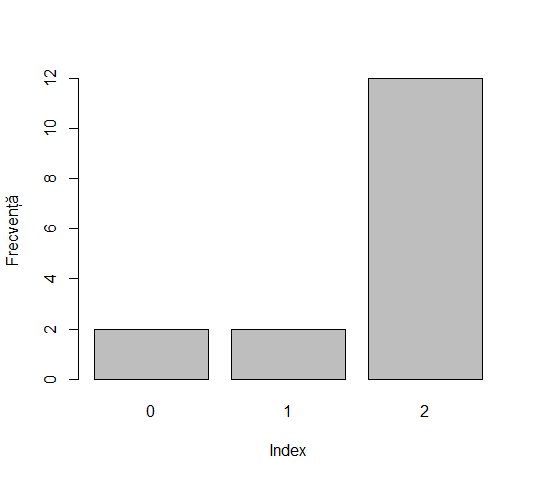
\includegraphics[width=0.75\linewidth]{CityPlatformPlot.png} \par
\caption{Histogramă a unei secvențe de etichete folosite la antrenare}
\end{figure}


\vspace{10mm}
\begin{figure}[H]
\centering
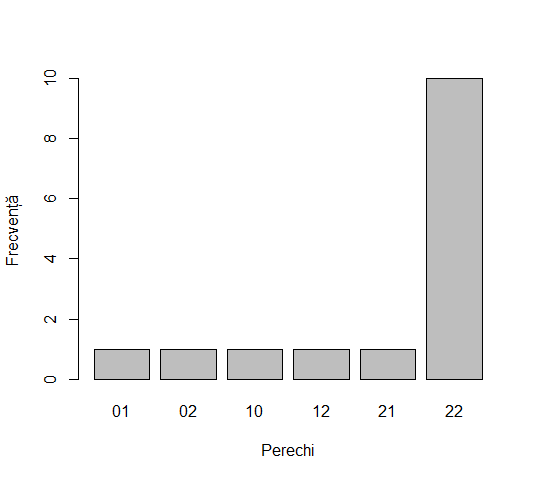
\includegraphics[width=0.75\linewidth]{CityPlatformPairPlot.png} \par
\caption{Histogramă a perechilor de etichete din secvența folosită la antrenare}
\end{figure}


Această soluție se bazează foarte mult pe calculul matriceal de accea în cadrul aplicației am fost nevoit să apelez la o librărie ce este folosită pentru calcul numeric. Deoarece acest algoritm se bazează foarte mult pe matrici, o incercare de implementare folosind unități de procesare grafice ar putea îmbunătăți substanțial viteza de convergență a algoritmului datorită puterii mai mari de calcul.\par

Parametri $\textbf{A},\textbf{B},\pi$ sunt initializați random și normalizați pe linii, iar apoi este calculat $\bar{C} = B\bar{A}B^{T}$, unde $\bar{A} = {\pi_{k}\cdot a_{kl}}, 1 \leq k \leq N, 1\leq l \leq N$. Următorul pas este calcularea matricii $R$ prin împărțirea element cu element a matricii $C$ la matricea $\bar{C}$.\par

După calculul acestor matrici intermediare urmează actualizare paremetrilor după urmatoarele ecuații preluate din publicație, $\bar{A'} = \bar{A} \odot B^{T}RB$  si $B' = B \odot(RB\bar{A}^{T} + R^{T}B\bar{A})$, unde $\odot$ reprezintă înmulțirea element cu element a două matrici. După acest calcul se face actualizarea astfel $A = norm(\bar{A'}),B = norm(B')$, unde $norm$ este o funcție ce realizează normalizarea pe toată matricea $A$ iar pentru $B$ doar pe coloane.\par

Acești pași se realizează pănă un anumit criteriu de convergență este satisfăcut. De obicei aceste criterii includ ca norma matricilor $A,B$ să fie sub un anumit epsilon împreună cu funcția de $log-likelihood$. În implementarea acestui algoritm am folosit ca și criterii de convergență, cum sugera și publicația de unde am preluat ideea, calcularea unei norme de tip $L^{2}$ aplicată matricilor $A,B,R$, ce ar trebui sa fie sub un $\epsilon = 10^{-6}$ și un număr maxim de iterații pentru care ar trebui să fie îndeplinită. Bineînțeles aceste condiții sunt doar cele standard, ele putând fi ușor schimbate în funcție de necesitate.\par

\section{Limitări ale modelului}

În secțiunile anterioare am văzut avantajele modelului Markov cu stări invizibile dar acesta suferă de o mare problemă, blocarea într-un optim local. Din cauza acestei probeleme estimarea de parametri este o sarcină destul de dificilă și delicată. De asemenea modelul depinde foarte mult de proprietatea Markov ce specifică clar că o stare viitoare poate să depindă doar de starea curentă, limitănd astfel capacitatea de a modela date mult mai complexe. Se poate extinde modelul la ultimele $n-1$ stări dar complexitatea de antrenare și durata crește considerabil.
\par

Cea mai simplă soluție pentru a preveni blocarea este inițializarea random a parametrilor modelului și reantrenarea lui de mai multe ori, pastrandu-se cel mai bun rezultat. Acestă soluție este fezabilă deoare prin randomizare se pot obține parametri din vecinătatea soluției optime, scăzănd posibilitatea ca algoritmul să ramană blocat într-un optim local, atunci cănd există o multitudine de aceste puncte. Deși această soluție rezolva problema în unele situații reantrenarea de foarte multe ori este costisitoare, de accea există posibilitatea de a salva parametri estimați, putănd fi ulterior utilizați de model prin o simplă citire.\par

\vspace{10mm}
\begin{figure}[H]
\centering
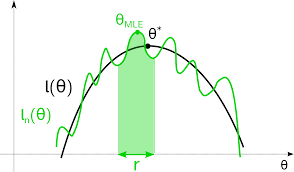
\includegraphics[width=0.4\linewidth]{MLE.png} \par
\caption{Grafic al functie $log-likelihood$ cu foarte multe puncte de optim local}
\end{figure}

Din cauza acestor limitări algoritmii de estimare a parametrilor precum $Baum-Welch$ nu garantează găsirea optimului global. Deseori un optim local este suficient pentru probleme ce nu necesită soluția optimă dar trebuie luat in considerare acest aspect atunci când se utiliează un astfel de algoritm.\par

O altă problemă a acestei abordări este că in general este asumată independența etichetelor una față de celălaltă limitănd astfel flexibilitatea modelului și capacitatea de modelare a datelor.\par

\section{Complexitate și metode de optimizare}
În acestă secțiune se vor prezenta problem legate de complexitatea algoritmului de antrenare căt și a algoritmului de eșantionare dintr-o distribuție de probabilitate discretă. Conform publicației algoritmul de estimare a parametrilor prezentat anterior ce foloseste de o matrice de apariție $C$ are complexitatea timp de ordinul $O(IM^{2}N + T)$\par, unde $I$ reprezintă numărul de iterații până la convergență.\par

Comparativ cu algoritmul $Baum-Welch$ ce are ca si complexitate timp $O(IN^{2}T)$ iar în practică secvența de etichete pe care e antrenat algoritmul are o lungime considerabil mai mare decăt cardinalul mulțimii $V$, adică $M$, de unde se observă că abordarea cu matricea de apariție aduce un surplus de rapiditate de procesare ce este important în domeniul jocurilor unde viteza este foarte importantă pentru a nu îngreuna procesul de randare și mulți alți factori de care este influențat un joc complex.\par

Legat de procesul de eșantionare, acesta este realizat prin calcularea distribuției $CDF$\footnote{Cumulative Distribution Function} pentru parametri $A,B$ ce mai apoi sunt sortate în ordine crescătoare pe linii pentru a putea realiza o căutare binară a stării către care se va face tranziția fiind dat un număr generat pseudorandom.Din punct de vedere al complexității sunt necesari pași adiționali cum ar fi sortarea și stocarea valorilor cumulative dar asta se face în etapa de inițializare avănd efect minimal asupra jocului. Ce se poate spune totuși de această abordare este că timpul de cautare a stării se transforma din $O(N)$, unde $N$ repezintă numărul de stări, în $O(log(N))$. Această optimizare este importantă deoarece operația de eșantionare are loc de zeci de ori pentru o platformă fiind practic cea mai folosită operație din cadrul librăriei.\par

Deși în practică metoda de $sampling$ în timp de $O(log(N))$ s-a dovedit a fi suficientă, există un algoritm și mai eficient decăt cel prezentat ce reușeste sa determine starea sau emisia find dat un număr generat random în timp de $O(1)$, avănd aceiași complexitate la inițializare căt și memorie ca și algoritmul de căutare binară.\par

Acest algoritm se numește \textit{metoda lui Alias}, și reușeste să obțina cea mai bună viteză posibilă pentru eșantionarea dintr-o distribuție de probabilitate discretă. În general ideea din spatele algorimlui este de a crea o altă distribuție pe baza celei de la intrare ce permite eșantionare în timp constant.\par

    \chapter{Aspecte teoretice}
Facilisi nullam vehicula ipsum a arcu. Purus semper eget duis at tellus at. Adipiscing tristique risus nec feugiat. Eu volutpat odio facilisis mauris sit. Porta nibh venenatis cras sed. Penatibus et magnis dis parturient. Sollicitudin aliquam ultrices sagittis orci a. Senectus et netus et malesuada fames ac turpis egestas integer. Cras tincidunt lobortis feugiat vivamus at augue eget arcu dictum. Leo vel fringilla est ullamcorper eget nulla facilisi etiam dignissim. Nulla aliquet enim tortor at auctor urna nunc id cursus. Elit duis tristique sollicitudin nibh. Sagittis nisl rhoncus mattis rhoncus urna neque viverra. Convallis posuere morbi leo urna molestie at. Quisque egestas diam in arcu cursus euismod.

\section{Titlul secțiunii 1}

A diam sollicitudin tempor id eu nisl. Hac habitasse platea dictumst vestibulum. Integer enim neque volutpat ac tincidunt. Facilisi nullam vehicula ipsum a arcu cursus vitae congue. Vel turpis nunc eget lorem. Vestibulum mattis ullamcorper velit sed ullamcorper morbi tincidunt ornare. Nunc sed blandit libero volutpat. Sit amet luctus venenatis lectus magna fringilla urna porttitor. Hac habitasse platea dictumst quisque sagittis purus. Sed faucibus turpis in eu mi bibendum neque egestas. Vel orci porta non pulvinar neque laoreet suspendisse interdum consectetur. Erat nam at lectus urna duis convallis convallis tellus id. Tristique sollicitudin nibh sit amet commodo nulla facilisi nullam vehicula. Etiam dignissim diam quis enim lobortis scelerisque. Nunc congue nisi vitae suscipit tellus mauris a diam maecenas. Lacus viverra vitae congue eu consequat ac felis donec. Mauris sit amet massa vitae tortor condimentum. Mauris augue neque gravida in. Lorem ipsum dolor sit amet. Arcu dui vivamus arcu felis bibendum ut tristique et.

\section{Titlul secțiunii 2}

Sit amet mauris commodo quis imperdiet massa tincidunt nunc pulvinar. Ligula ullamcorper malesuada proin libero nunc consequat interdum. Mauris a diam maecenas sed enim ut. Ut sem nulla pharetra diam sit amet nisl suscipit adipiscing. Leo duis ut diam quam nulla. Neque ornare aenean euismod elementum. Vitae sapien pellentesque habitant morbi tristique senectus. Lectus magna fringilla urna porttitor rhoncus dolor purus non enim. Egestas sed sed risus pretium quam vulputate dignissim suspendisse in. At quis risus sed vulputate odio ut enim. Hac habitasse platea dictumst quisque sagittis. Lectus vestibulum mattis ullamcorper velit sed. Massa vitae tortor condimentum lacinia quis vel eros donec ac. Vulputate dignissim suspendisse in est ante. Sed faucibus turpis in eu mi bibendum neque. Enim eu turpis egestas pretium aenean pharetra magna. Tellus mauris a diam maecenas.

\section{Titlul secțiunii 3}

Faucibus ornare suspendisse sed nisi lacus sed. Mi in nulla posuere sollicitudin aliquam ultrices. Lacus suspendisse faucibus interdum posuere lorem ipsum dolor sit amet. Odio tempor orci dapibus ultrices in iaculis nunc sed augue. Congue eu consequat ac felis donec et odio. Enim ut sem viverra aliquet eget sit amet. Sit amet consectetur adipiscing elit duis tristique sollicitudin. Quis blandit turpis cursus in. Cras fermentum odio eu feugiat pretium nibh ipsum consequat nisl. Non curabitur gravida arcu ac tortor dignissim convallis aenean. Porta non pulvinar neque laoreet suspendisse interdum consectetur libero id. Lacus viverra vitae congue eu consequat ac felis. Vulputate dignissim suspendisse in est ante in nibh mauris. Amet mauris commodo quis imperdiet massa. Varius sit amet mattis vulputate enim nulla aliquet. Pellentesque diam volutpat commodo sed egestas egestas. Amet est placerat in egestas erat imperdiet sed euismod. Scelerisque varius morbi enim nunc faucibus a pellentesque sit. Ut sem viverra aliquet eget sit amet tellus cras. Sem integer vitae justo eget magna fermentum iaculis eu.
    \chapter{Arhitectura aplicației}

Amet venenatis urna cursus eget. Quam vulputate dignissim suspendisse in est ante. Proin nibh nisl condimentum id. Egestas maecenas pharetra convallis posuere morbi. Risus viverra adipiscing at in. Vulputate eu scelerisque felis imperdiet. Cras adipiscing enim eu turpis egestas pretium aenean pharetra. In aliquam sem fringilla ut morbi tincidunt augue. Montes nascetur ridiculus mus mauris. Viverra accumsan in nisl nisi scelerisque eu ultrices vitae. In nibh mauris cursus mattis molestie a iaculis. Interdum consectetur libero id faucibus nisl tincidunt eget. Gravida in fermentum et sollicitudin ac orci. Suscipit adipiscing bibendum est ultricies. Etiam non quam lacus suspendisse. Leo urna molestie at elementum eu facilisis sed odio morbi. Egestas congue quisque egestas diam in arcu cursus. Amet consectetur adipiscing elit ut aliquam purus.
    
    \chapter*{Concluzii} 
\addcontentsline{toc}{chapter}{Concluzii}
    \chapter*{Bibliografie} 
\addcontentsline{toc}{chapter}{Bibliografie}
\section{Cărți și Articole}
\begin{itemize}
    \item{Madhusudana Shashanka, \textit{A Fast Algorithm For Discrete HMM Training Using Observed Transitions},\newline \url{https://pdfs.semanticscholar.org/9c19/af77335ee1e28875b84eeb0b8c71daa9fdf3.pdf}}
    \item{Gleidson Mendes Costa, Tiago Bonini Borchartt,\newline \textit{Procedural terrain generator for platform games using Markov chain
}, 2018,  \url{http://www.sbgames.org/sbgames2018/files/papers/ComputacaoShort/188123.pdf}}
	\item{Fanny Yang,Sivaraman Balakrishnan, Martin J. Wainwright,\newline \textit{Statistical and Computational Guarantees for the
Baum-Welch Algorithm}, 2015,\newline \url{https://arxiv.org/pdf/1512.08269.pdf}}
	\item{Sam Snodgrass, Santiago Ontañón,\newline \textit{Experiments in Map Generation using Markov Chains},2014,\newline \url{http://fdg2014.org/papers/fdg2014_paper_29.pdf}}
	\item {Liviu Ciortuz, \textit{Machine Learning Course},\newline \url{https://profs.info.uaic.ro/~ciortuz/SLIDES/hmm.pdf}}
	\item{\textit{Unity User Manual},\newline \url{https://docs.unity3d.com/Manual/index.html}}
\end{itemize}

\section{Obiecte preluate și folosite în cadrul aplicației}
\begin{itemize}
    \item{Unity Asset Store, \textit{Low Poly European City Pack},\newline \url{https://assetstore.unity.com/packages/3d/environments/urban/low-poly-european-city-pack-71042}}
	\item{Unity Asset Store, \textit{Low Poly Desert Pack},\newline \url{https://assetstore.unity.com/packages/3d/environments/free-low-poly-desert-pack-106709}}
	\item{Unity Asset Store, \textit{Low Poly Police Car 01},\newline \url{https://assetstore.unity.com/packages/3d/vehicles/land/low-poly-police-car-01-142826}}
	\item{Unity Asset Store, \textit{Low Poly Destructible 2 Cars No.8},\newline \url{https://assetstore.unity.com/packages/3d/vehicles/land/low-poly-destructible-2-cars-no-8-45368}}
	\item{Unity Asset Store, \textit{PBR Dirty Dumpster},\newline \url{https://assetstore.unity.com/packages/3d/props/exterior/pbr-dirty-dumpster-59840}}
	\item{Unity Asset Store, \textit{Unity Particle Pack 5.x},\newline \url{https://assetstore.unity.com/packages/essentials/asset-packs/unity-particle-pack-5-x-73777}}
	\item{Unity Asset Store, \textit{Post Processing Stack},\newline \url{https://assetstore.unity.com/packages/essentials/post-processing-stack-83912}}
	\item{Joao Paulo, \textit{Low Poly Farm},\newline \url{https://3dshed.wordpress.com/2018/08/29/low-poly-farm-animation/}}
	\item{Joao Paulo, \textit{Wind Turbine},\newline \url{https://3dshed.wordpress.com/2018/02/12/wind-turbine-001-animated/}}
	\item{Joao Paulo, \textit{Trees Pack},\newline \url{https://3dshed.wordpress.com/2018/04/07/trees-pack-001/}}
	\item{Joao Paulo, \textit{Desert Texture},\newline \url{https://3dtextures.me/2018/08/13/cracked-mud-001/}}
	\item{Joao Paulo, \textit{Asphalt Texture},\newline \url{https://3dtextures.me/2018/05/07/asphalt-005/}}
	\item{Joao Paulo, \textit{Stone Tile Texture},\newline \url{https://3dtextures.me/2018/09/27/stone-tiles-003/}}
	\item{Joao Paulo, \textit{Grass Texture},\newline \url{https://3dtextures.me/2018/01/05/grass-001-2/}}
	\item{SlightlyMad, \textit{Volumetric Lights},\newline \url{https://github.com/SlightlyMad/VolumetricLights}}
	\item{DavidMenke, \textit{Main Menu Sound},\newline \url{https://freesound.org/people/davidmenke/sounds/319750/}}
	\item{Kenney.nl, \textit{Buttons Effects},\newline \url{https://opengameart.org/content/51-ui-sound-effects-buttons-switches-and-clicks}}
	\item{\textit{Borg Font},\newline \url{https://www.dafont.com/borg.font}}
\end{itemize}

\end{document}
